\begin{enumerate}[label=\thesection.\arabic*.,ref=\thesection.\theenumi]
\numberwithin{equation}{enumi}

\item
For a system having transfer function G(s) = $\frac{-s+1}{s+1}$ 
,a unit step input is applied  at t = 0 .The value of the system at t =1.5 sec is
\newline
\ Solution: 
\newline
Given x(t) = u(t) a unit step signal .The Laplace transform of x(t) is:
\begin{align}
X(s) = \int_{0}^{\infty}x(t) e^{-st} dt
\end{align}
\begin{align}
   X(s) = \frac{1}{s}
\end{align}
In Laplace domain ,
\begin{align}
     Y(s) = X(s)G(s)
\end{align}
\begin{align}
    Y(s) = \frac{-s+1}{s(s+1)}
\end{align}
By doing partial fractions ,
\begin{align}
    Y(s) = \frac{1}{s} -\frac{2}{s+1}
\end{align}

The inverse Laplace transform of Y(s) is,
\begin{align}
    y(t) = u(t) - 2e^{-t}u(t)
\end{align}
y(t) at t = 1.5sec
\begin{align}
    y(1.5) = 0.55
\end{align}
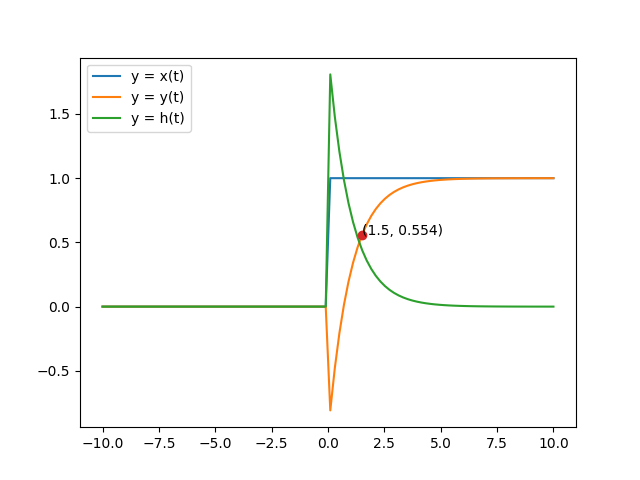
\includegraphics[width=1\linewidth]{plotting of functions.png} 
\begin{figure}[!ht]

 %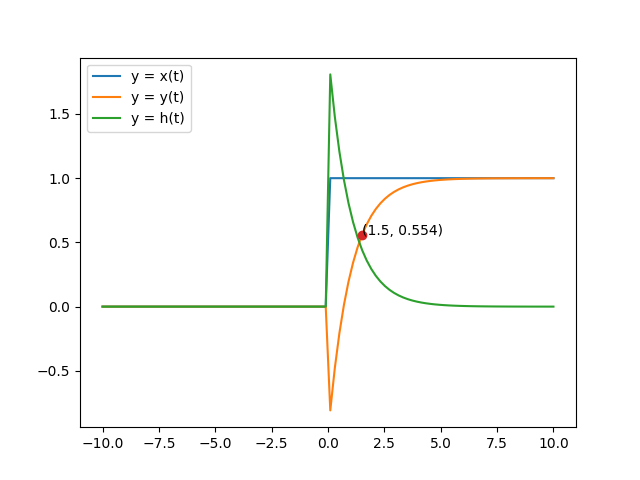
\includegraphics[width=1\linewidth]{plotting of functions.png} 
  \centering
  
    
    \label{fig;Graph}
\end{figure}
\item  Python code for below graph
\begin{1stlisting}
codes/ee18btech11042/graph plot.py
\end{1stlisting}

    
\end{enumerate}

    © 2020 GitHub, Inc.
    Terms
    Privacy
